
\begin{figure}[H]
\centering
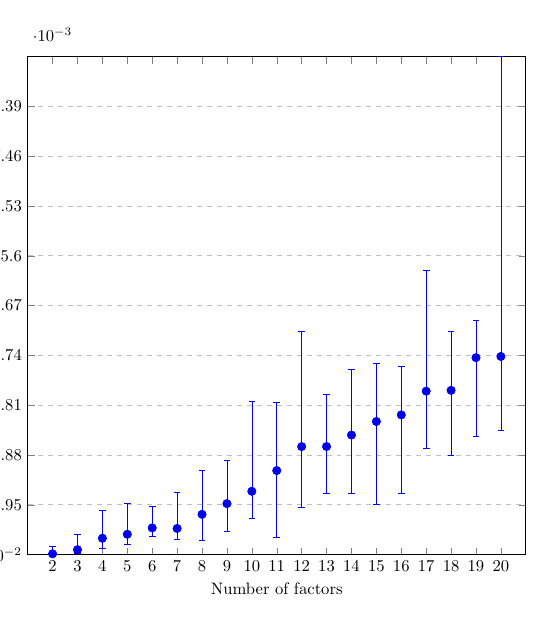
\begin{tikzpicture}[scale=0.6, trim axis left, trim axis right]
\begin{axis}[
    width=1\textwidth,
    height=1\textwidth,
    xlabel={Number of factors},
    ylabel={Time taken (s)},
    xmin=1.0, xmax=21.0,
    ymin=1.9e-05, ymax=0.009317,
    xticklabels={2, 3, 4, 5, 6, 7, 8, 9, 10, 11, 12, 13, 14, 15, 16, 17, 18, 19, 20},
    xtick={2, 3, 4, 5, 6, 7, 8, 9, 10, 11, 12, 13, 14, 15, 16, 17, 18, 19, 20},
    ytick={1.9e-05, 0.0009488, 0.0018786, 0.0028084, 0.0037382, 0.004668, 0.0055978, 0.0065276, 0.0074574, 0.0083872},
    ymajorgrids=true,
    grid style=dashed,
]

\addplot+[
    blue,
    very thick,
    forget plot,
    only marks
    ]
    plot[
    very thick,
    error bars/.cd,
    y dir=plus,
    y explicit
    ]
    table[x=x,y=y,y error expr=\thisrow{y-max}] {
    x    y    y-max
    11	0.0015875125	0.0012754875
10	0.0012010125	0.0016709875
13	0.002036125	0.000979875
12	0.0020351	0.0021599
15	0.002503125	0.001089875
14	0.002250675	0.001235325
17	0.0030697125	0.0022602875
16	0.0026267125	0.0009122875
19	0.0036951125	0.0007028875
18	0.0030848125	0.0010931875
20	0.0037176625	0.0055993375
3	0.0001103875	0.0002796125
2	3.39e-05	0.0001341
5	0.00039845	0.00058655
4	0.0003240375	0.0005159625
7	0.0005071375	0.0006688625
6	0.000517675	0.000393325
9	0.00097005	0.00080495
8	0.0007702875	0.0008277125

    };

\addplot+[
    blue,
    very thick,
    forget plot,
    only marks
    ]
    plot[
    very thick,
    error bars/.cd,
    y dir=plus,
    y explicit
    ]
    table[x=x,y=y,y error expr=\thisrow{y-min}] {
    x    y    y-min
    11	0.0015875125	-0.0012555125
10	0.0012010125	-0.0005090125
13	0.002036125	-0.000870125
12	0.0020351	-0.0011361
15	0.002503125	-0.001550125
14	0.002250675	-0.001081675
17	0.0030697125	-0.0010707125
16	0.0026267125	-0.0014727125
19	0.0036951125	-0.0014611125
18	0.0030848125	-0.0012128125
20	0.0037176625	-0.0013776625
3	0.0001103875	-5.93875e-05
2	3.39e-05	-1.49e-05
5	0.00039845	-0.00018945
4	0.0003240375	-0.0001810375
7	0.0005071375	-0.0001991375
6	0.000517675	-0.000158675
9	0.00097005	-0.00051205
8	0.0007702875	-0.0004912875

    };

\end{axis}
\end{tikzpicture}
\vspace{-0.3cm}
\caption{Small primes, close primes}\label{fig:PollardsRhoAlgorithmSmallcloseprimesfactors}
\end{figure}

